% Created 2015-10-23 Fri 17:36
\documentclass{scrartcl}
\usepackage[utf8]{inputenc}
\usepackage[T1]{fontenc}
\usepackage{fixltx2e}
\usepackage{graphicx}
\usepackage{longtable}
\usepackage{float}
\usepackage{wrapfig}
\usepackage{soul}
\usepackage{textcomp}
\usepackage{marvosym}
\usepackage{wasysym}
\usepackage{latexsym}
\usepackage{amssymb}
\usepackage{hyperref}
\tolerance=1000
\usepackage{khpreamble}
\newcommand{\tustin}{\ensuremath{\frac{2}{h}\frac{z-1}{z+1}}}
\providecommand{\alert}[1]{\textbf{#1}}

\title{Computerized control - partial exam 2 (20\%)}
\author{Kjartan Halvorsen}
\date{2015-10-23}
\hypersetup{
  pdfkeywords={},
  pdfsubject={},
  pdfcreator={Emacs Org-mode version 7.9.3f}}

\begin{document}

\maketitle


\section*{Problem 1}
\label{sec-1}

  In the preparation exercise for this exam a controller was designed for the system 
  \[ G(s) = \frac{1}{s}\left(\frac{-s+2}{s+2}\right)\]
  which has a zero in the right half plane. The continuous-time controller was given by the transfer function 
  \[ F(s) = 3\frac{s+2}{s+8}. \]
\begin{enumerate}
\item Sample the controller using Tustin's approximation \[s=\tustin.\]
\item Show that the discrete controller is stable for all choices of sampling period $h$.
\item The cross-over frequency of the continuous-time open loop transfer function was found to be $\omega_c=\unit{0.8}{\rad\per\sec}$. What is the phase of the continuous-time controller at this frequency (what is its complex argument)?
\item Will the open-loop system using the sampled controller you obtained have a phase margin which is greater than or less than the phase margin using the continuous-time controller? Motivate your answer!
\end{enumerate}
\section*{Problem 2}
\label{sec-2}

  In figure \ref{fig:bode} the open-loop transfer function for the system in Problem 1 with a discrete controller ($h=0.2$) is given. Identify (mark in the figure):
\begin{enumerate}
\item The cross-over frequency $\omega_c$.
\item The phase margin $\varphi_m$.
\item The phase-cross over frequency $\omega_p$.
\item The amplitude margin $A_m$.
\end{enumerate}

  \begin{figure}
  \begin{center}
  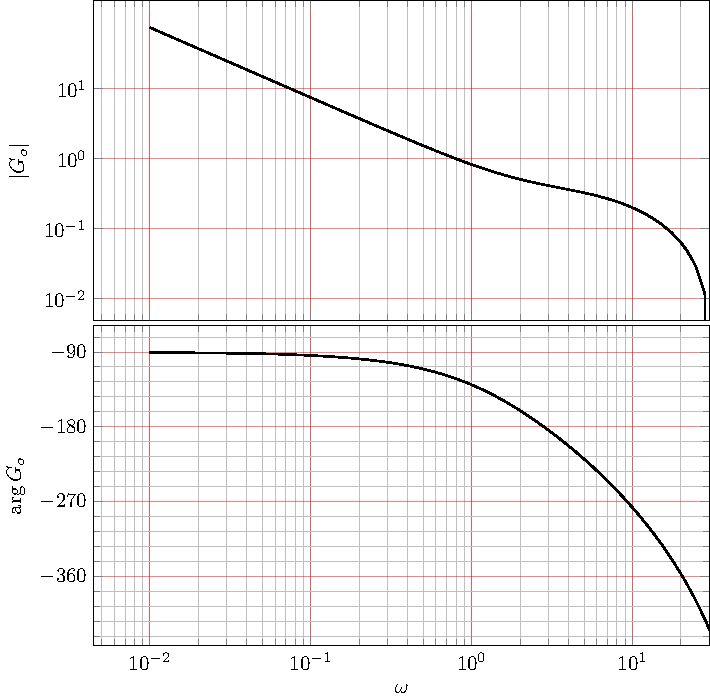
\includegraphics[width=0.8\linewidth]{bode-openloop-exam}
  \caption{Bode diagram of open-loop transfer function.}
  \label{fig:bode}
  \end{center}
  \end{figure}
\section*{Solutions}
\label{sec-3}
\subsection*{Problem 1}
\label{sec-3-1}

\begin{enumerate}
\item The sampled controller using Tustin's approximation becomes
      \[F_d(z) = F(s')|_{s'=\tustin} = 3 \frac{\tustin + 2}{\tustin + 8} = 3 \frac{(1+h)z-(1-h)}{(1+4h)z-(1-4h)}. \]
\item The characteristic equation of the discrete controller is
      \[ (1+4h)z-(1-4h) = 0. \]
      Clearly, the controller has a single pole in $\frac{1-4h}{1+4h}$ which is inside the unit disk for all positive values of $h$.
\item The phase of the controller at $\omega_c = 0.8$ is 
      \[\arg F(i\omega_c) = \arg (i\omega_c + 2) - \arg (i\omega_c + 8) = \arctan \frac{0.8}{2} - \arctan \frac{0.8}{8} \approx \unit{0.28}{\rad} = \unit{16.1}{\degree}. \]
\item The sampled controller will have a phase margin which is \textbf{smaller} than that of continous-time system,  since the sample-and-hold of the discrete controller introduces a time-delay of about half the sampling period. More argumentation than this is not necessary for full points. But for the interested: In the case with $h=\unit{0.2}{\sec}$, the (approximate) time-delay is \unit{0.1}{\sec} and the corresponding phase contribution of the sample-and-hold at the cross-over frequency is
      \[ \arg \mexp{-i0.1\omega_c} = \unit{-0.08}{\rad} \approx \unit{-4.58}{\degree}. \]
      We can also find this by considering the transfer function of the zero-order-hold block, which is given by
      \[ \frac{1}{s}\big(1-\mexp{-sh}\big). \]
      The phase contribution of this block at $\omega_c$ is given by
      \begin{equation*}
      \begin{split}
       \arg \big(1-\mexp{-i\omega_ch}\big)\frac{1}{i\omega_c} &= \arg \big(1-\mexp{-i0.16}\big) - \arg i0.8\\
      &= \arg \big(1-\cos(-0.16) -i\sin(-0.16)\big) - \pi/2\\ &= \arctan \frac{\sin(0.16)}{1-\cos(0.16)} - \pi/2 = \unit{-0.08}{\rad} \approx \unit{-4.58}{\degree}.
      \end{split}
      \end{equation*}
\end{enumerate}
\subsection*{Problem 2}
\label{sec-3-2}

   \begin{center}
   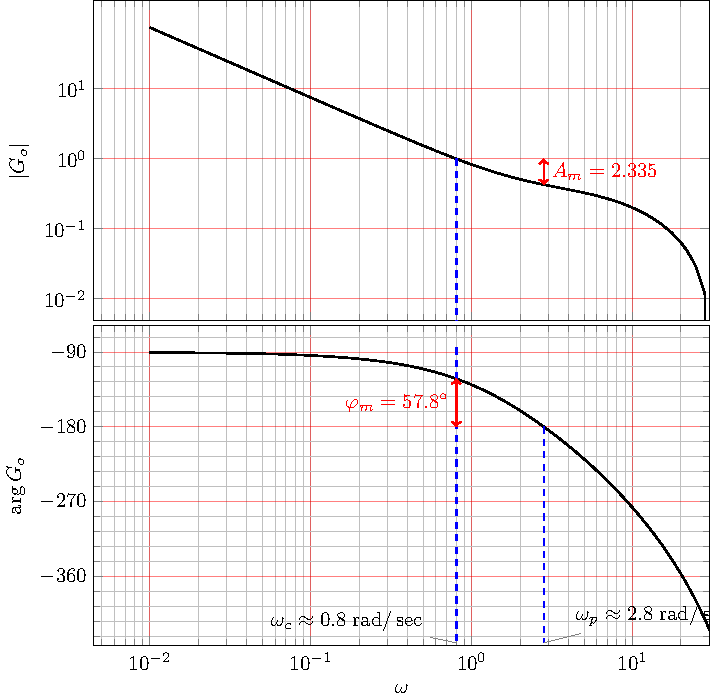
\includegraphics[width=0.8\linewidth]{bode-openloop-exam-solution}
   \end{center}

\end{document}
